\documentclass[10pt]{article}
\usepackage[portrait]{geometry}

\usepackage{biblatex}
\addbibresource{bibliography.bib} % Ensure this matches the name of your .bib file.

%=============================================================================
%   Packages
%=============================================================================

\usepackage{graphicx} % Required for inserting images
\usepackage{enumerate} % Useful if you need to customize enumerated lists, like when writing out an algorithm
\usepackage{amsfonts, mathrsfs} % Useful fonts for mathematics writing
\usepackage{amsmath} % A basic package for mathematical typesetting, useful for equations
\usepackage{amsthm} % Provides the ability to write formatted lemmas, theorems, etc.
\usepackage{tikz} % The functionality for drawing graphs if you want to write them by hand (very powerful and flexible, but tricky)
\usepackage{tikz-cd} % The functionality for drawing graphs if you use the website shown below to draw them as needed
\usetikzlibrary{calc, angles, quotes}
\usepackage{adjustbox} % Useful for modifying the size of various things.
\usepackage{hyperref} % Allows equation and figure labels to be hyperlinks in your document, by default

%=============================================================================
%   User Defined Commands
%=============================================================================

% Defining your own commands and shorthands can be greatly convenient.
\newcommand{\pderiv}[2]{\frac{\partial #1}{\partial #2}}
\newcommand{\R}{\mathbb{R}}

% See https://www.overleaf.com/learn/latex/Theorems_and_proofs for an excellent overview of defining theorem environments}
\newtheorem{theorem}{Theorem}[section]
\newtheorem{cor}{Corollary}

%=============================================================================
%   The Start
%=============================================================================

\title{Mathematical Innovations and Applications in Chinese History: An Analysis of \textit{The Nine Chapters on the Mathematical Art}}
\author{Wentao Jiang}
\date{Spring 2024}

\begin{document}

\maketitle

\section{Introduction}

\textit{The Nine Chapters on the Mathematical Art} is a practical handbook of mathematics. It stands as a landmark to the mathematical sophistication of ancient Chinese academia. Assembled during the Han Dynasty, it encompasses a wide range of mathematical problems from practical everyday life, reflecting the era's economic and administrative needs \autocite{Kangshen_Crossley}.

\vspace{7pt}

This paper explores the specific applications of geometry as detailed in chapters crucial to agriculture, construction, taxation, and astronomy. These chapters offer a concise mathematical perspective on how ancient Chinese civilization utilized mathematics as a tool for governance, societal organization, and advancement.
\vspace{7pt}

The Han Dynasty bore witness to the standardization of weights and measures, manifesting the pivotal role of mathematics in unifying the empire. The Historical Context and \textit{The Nine Chapters on the Mathematical Art} \autocite{Kangshen_Crossley} captures the essence of this period through its discourse on the state’s imperative for precise land measurement, resource allocation, and the monumental architectural feats of the time.

\vspace{7pt}

Chapter 1, \textbf{Field Measurement}, lays the groundwork for our discussion on the Geometry of Agriculture and Taxation. This chapter details the measurement of land for agricultural purposes, an essential activity with direct tax implications. Building upon this, Chapter 6, \textbf{Fair Levies}, elaborates on the geometric methods employed for equitable taxation, revealing their significance within the economic fabric of the time.

\vspace{7pt}

Chapter 9, \textbf{Right-Angled Triangles}, transcends the earthly applications of geometry, towards the universe. This chapter serves as the foundation for our Astronomical and Calendar Calculations section, demonstrating how geometry informed the making of calendars and the understanding of the cosmos, and how ancient Chinese played a role in celestial observations and the development of a calendar system, crucial for both agriculture and the divination practices of the time.

\vspace{7pt}

In this study, the chosen sections draw upon the profound mathematical methodologies illustrated in \textit{The Nine Chapters on the Mathematical Art} \autocite{Kangshen_Crossley} to underscore the intrinsic role of mathematics in shaping the societal and cultural paradigms of the time, between mathematical advancements and the narrative arc of Chinese civilization.

\vspace{7pt}

Subsequent sections aim to deepen our exploration into the historical and their enduring legacy and the threads of influence these mathematical principles had on the era's culture and economy. Through a critical examination of its content and impact, we seek to elucidate the significant ways in which this mathematical treatise influenced the trajectory of Chinese mathematical practice and, by extension, its broader societal implications.

\vspace{10pt}

\section{Practical Geometry in Ancient China: Insights from \textit{The Nine Chapters}}

\vspace{7pt}

\subsection{Field Measurement and Standard Units (Chapter 1 \& 6)}

In the vast landscape of ancient China, the management of agricultural land was not only an economic activity but also a reflection of the civilization's mathematical sophistication. \textit{The Nine Chapters on the Mathematical Art} provides a window into this world, which delve into the realms of field measurement and fair levies, encapsulated within Chapters 1 and 6.

\vspace{7pt}

Field Measurement is delineated as the application of geometric principles to accurately determine agricultural land areas. This process is essential for assessing land parcels, facilitating a systematic approach to land division, management, and taxation.

\vspace{5pt}

Specific Standard Units are also employed in \textit{The Nine Chapters on the Mathematical Art}, including \textit{bu} for length and \textit{mu} for area, with 1 \textit{mu} being equivalent to 240 square \textit{bu} in Han Dynasty. Other units include \textit{kui}, \textit{su}, among others. The consistency in land assessment and taxation across the empire, underscores the importance of uniform measurement systems in ancient bureaucratic practices. \autocite[p.~191]{Martzloff_2006}

\vspace{5pt}

The geometric determination of land areas has a direct influence on taxation, where taxes should be proportionally levied based on precise measurements of land with emphasis on an early commitment to fairness and equity in economic policies. Furthermore, this approach highlights the role of geometry in establishing a just system for tax allocation by ensuring that land measurements and thus tax calculations are based on precise and verifiable data. By grounding tax calculations in the objective measurement of land, ancient practices underscored the importance of mathematical accuracy in supporting equitable economic structures.

\vspace{5pt}

For a rectangular field with known length \( l \) and breadth \( b \), its area \( A \) is given by the formula \( A = l \times b \). While rectangular fields allow for simple area calculations, ancient Chinese mathematicians also developed methods for dealing with irregularly shaped parcels of land. Techniques involved subdividing complex shapes into a combination of simpler geometric figures, for which areas could be individually calculated and then aggregated. 


\vspace{7pt}

Although the concept of functions, as understood in modern mathematics, does not explicitly appear in The \textit{Nine Chapters on the Mathematical Art}, the relationships between quantities could be considered early examples of functions. The approach to solving the systematic methods suggest an intuitive understanding of some concepts that underlie the modern concept of functions. In modern language, we can assume the following function, reference to the practical problem-solving methods in Chapter 6.

\vspace{10pt}

\textbf{Proposition 2.1.1}: Building on the historical insights from \textit{The Nine Chapters on the Mathematical Art}, we propose a mathematical model that reflects the ancient Chinese methods of land taxation and productivity assessment. This model introduces a function, denoted by \( T = f(r, A, w, g) \), dynamically mapping the area of land (\( A \)) to an appropriate tax amount (\( T \)) by incorporating variables such as the base tax rate (\( r \)), work coefficient (\( w \)), and geometric factor (\( g \)). This function aims to capture the nuanced approach to tax assessment typical of ancient practices, accommodating variations in agricultural value and productivity potential across different lands.

\vspace{7pt}

The function is expressed mathematically as:
\[ T = f(r, A, w, g) = r \cdot A \cdot w \cdot g \]
Here, \( r \) represents the base tax rate established by empire authority, which standardizes the initial tax calculations across regions. \( A \) is the land area measured using advanced geometric techniques, critical for ensuring accurate and fair tax calculations. The work coefficient \( w \) reflects land fertility and productivity, with values above 1 indicating higher fertility. The geometric factor \( g \) adjusts for irregular land shapes, influencing the usable area and consequently, the tax valuation.

\vspace{7pt}

The accuracy of these measurements is crucial for ensuring the reliability of tax calculations, thereby promoting an equitable distribution of tax burdens among landowners. This model not only enhances the precision of tax assessments but also reflects a commitment to fairness and justice in taxation, echoing ancient values and practices.

\vspace{15pt}

\textbf{Proposition 2.1.2: Area of Isosceles Triangle (Refer to Figure 1):} 
Let us consider a field shaped as an isosceles triangle, denoted as ABC, with the segment BC serving as the base (or breadth) of the triangle. The unique properties of the isosceles triangle allow for a creative approach to determining its area, a technique inspired by ancient mathematical methods.


\vspace{7pt}

\vspace{20pt}
\begin{figure}[htbp]
\centering % This centers the entire figure environment

\begin{minipage}{0.5\textwidth}
  \centering % This centers the content inside the minipage
  % First tikzpicture starts here
  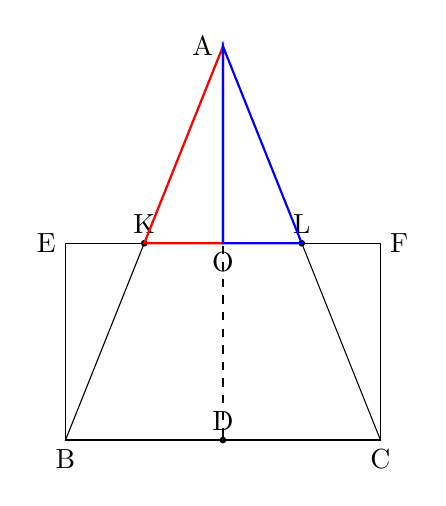
\begin{tikzpicture}[scale=1, every node/.style={scale=1}]
    % Define points
    \coordinate (A) at (2,5);
    \coordinate (B) at (0,0);
    \coordinate (C) at (4,0);
    \coordinate (E) at (0,2.5);
    \coordinate (F) at (4,2.5);
    
    % Draw triangle and rectangle
    \draw (A) -- (B) -- (C) -- cycle;
    \draw (B) rectangle (F);
    
    % Draw perpendicular bisector AD and midpoint O
    \draw[dashed] (A) -- node[right] {} ($(B)!(A)!(C)$) coordinate (D);
    
    \coordinate (O) at ($(E)!0.5!(F)$);
    \coordinate (K) at ($(E)!0.5!(O)$);
    \coordinate (L) at ($(O)!0.5!(F)$);
    \draw[fill=black] (D) circle(1pt) node[above] {D};
    \draw[fill=black] (K) circle(1pt) node[above] {K};
    \draw[fill=black] (L) circle(1pt) node[above] {L};
    
    % Draw areas to move
    \draw[red, thick] (A) -- (O) -- (K) -- cycle; % Triangle AOL
    \draw[blue, thick] (A) -- (O) -- (L) -- cycle; % Triangle AOK
    
    % Labels
    \node at (A) [left] {A};
    \node at (B) [below] {B};
    \node at (C) [below] {C};
    \node at (E) [left] {E};
    \node at (F) [right] {F};
    \node at (O) [below] {O};
  \end{tikzpicture}
  % First tikzpicture ends here
\end{minipage}\hfill 
\begin{minipage}{0.5\textwidth}
  \centering
  % Second tikzpicture starts here
  \begin{tikzpicture}[scale=1, every node/.style={scale=1}]
    % Define points
    \coordinate (B) at (0,0);
    \coordinate (C) at (4,0);
    \coordinate (E) at (0,2.5);
    \coordinate (F) at (4,2.5);
    
    % Draw rectangle
    \draw (B) rectangle (F);
    
    \coordinate (K) at ($(E)!0.5!(O)$);
    \coordinate (L) at ($(O)!0.5!(F)$);
    \draw[fill=black] (K) circle(1pt) node[above] {K};
    \draw[fill=black] (L) circle(1pt) node[above] {L};
    
    % Draw areas to move
    \draw[red, thick] (B) -- (K) -- (E) -- cycle;
    \draw[blue, thick] (C) -- (F) -- (L) -- cycle;
    
    % Labels
    \node at (B) [below] {B};
    \node at (C) [below] {C};
    \node at (E) [left] {E};
    \node at (F) [right] {F};
  \end{tikzpicture}
  % Second tikzpicture ends here
\end{minipage}

\caption{Illustration of calculating area of Triangle.}
\end{figure}

\vspace{20pt}

In our geometric construction, starting from the base BC of the triangle ABC, we extend lines to form the rectangle BCFE. We ensure that the height BE of the rectangle is precisely half the height AD of the triangle. The height AD acts as the perpendicular bisector, extending from the apex A and intersecting the rectangle's upper boundary at midpoint O. This construction  divides the entire height into manageable and symmetrical sections.

\vspace{7pt}

The next step involves a geometric manipulation: we reposition the triangular areas within our constructed shapes to form a perfect rectangle. Specifically, the surplus area within triangle AOL is moved to fill the deficit in triangle CFL, and similarly, the area within triangle AOK is used to fill the space in triangle BEK. Through this process of shifting and rearranging, we successfully transform the irregular triangular areas into a precise rectangle, EFCB. 

\vspace{7pt}

As a result, we can conclude that the area of triangle ABC is effectively congruent to the area of rectangle EFCB. This area is calculated as the product of half the length and the breadth of the rectangle, a method that simplifies the computation. 

\vspace{7pt}

This proposition draws direct parallels to Problem 26 from Chapter 1 of \textit{The Nine Chapters on the Mathematical Art}, where the principles of "half-width multiplied by straight length" and "complementing the void with the excess" are employed. These methods, as described by Kangshen et al.\autocite{Kangshen_Crossley}, showcase the ingenuity and practicality of ancient Chinese mathematicians in solving real-world problems through geometric transformations. By reviving these historical techniques, we not only validate their relevance but also provide a bridge linking ancient wisdom with modern mathematical practices.

\vspace{15pt}

\textbf{Proposition 2.1.3: Area of an Inscribed Dodecagon (Refer to Figure 2):}
Consider BC as a side of an inscribed hexagon within a circle, and HC as a side of the inscribed dodecagon, with AH denoting the circle's radius.

\begin{figure}[ht!]
\centering
\includegraphics[width=0.5\textwidth]{./images/sec2.1-dodecagon.jpeg}
\caption{Geometric Construction of an Inscribed Dodecagon.}
\label{fig:dodecagon}
\end{figure}

\vspace{7pt}

Drawing upon the rich mathematical tradition of \textit{The Nine Chapters on the Mathematical Art}, particularly to the focus on land measurement and the application of geometric principles to practical problems, this proposition explores the calculation of the area of a geometrically significant shape: the inscribed dodecagon. These chapters illustrate the use of geometric transformations and area calculations that are foundational to the methods employed here.

\vspace{7pt}

We propose that the area of an inscribed dodecagon can be calculated as three times the product of the radius (AH) and the length of one side of the inscribed hexagon (BC). This initially unintuitive claim is supported by historical methodologies that simplify complex geometric forms into calculable shapes, as outlined in Martzloff's discussion \autocite[p.~278]{Martzloff_2006}.

\vspace{7pt}

Geometrically, this can be demonstrated by constructing rectangle FGED, where the area is the product of BC and AH. By relocating triangles AHC and COH to fill the deficit areas in triangles AGC and CEH respectively, we transform this construction into a square AGEH. This process mirrors the ancient technique of "complementing the void with the excess," a principle that is extensively utilized in Chapter 6 to solve various practical geometry problems.

\vspace{7pt}

The transformation results in the area of square AGEH being twice that of triangle AHC, and hence, rectangle FGED is four times the area of triangle AHC. Since the dodecagon consists of 12 such triangles, the total area calculation confirms our proposition, tying directly back to the methods of systematic manipulation and calculation described in these pivotal chapters.

\vspace{7pt}

This proposition not only reinforces the contemporary relevance of ancient mathematical practices but also demonstrates the enduring utility of these techniques in solving modern-day problems, bridging historical insights with advanced geometric calculations. The proposition thus serves as a modern application of the principles documented in \textit{The Nine Chapters on the Mathematical Art} and demonstrates even more the timelessness of these mathematical innovations.

\vspace{15pt}

\textbf{Proposition 2.1.4: Equitable Land Allocation Based on River Flooding} In ancient China, managing agricultural land effectively, especially near rivers, was essential due to the enhanced fertility from periodic flooding. The equitable distribution of this fertile land was crucial for maximizing agricultural output and maintaining fairness among farmers. This proposition introduces a method to allocate land based on its proximity to a river, which directly influences its agricultural value.

\vspace{7pt}

The mathematical model for this allocation uses the following variables and formulas:
\begin{align}
    & \text{Let } d_i \text{ be the distance of strip } i \text{ from the river.} & \nonumber \\
    & \text{Let } l_i \text{ be the length of strip } i. & \nonumber \\
    & \text{Assume } f_i = \frac{1}{d_i} \text{ represents the fertility factor of strip } i, \text{ inversely proportional to } d_i. & \nonumber
\end{align}

The aim is to determine the length \(l_i\) of each land strip such that each has equal agricultural value, despite varying fertility due to their distances from the river:

\begin{align}
    & \text{The area } A_i = w \times l_i, \text{ where } w \text{ is the constant width of the strips.} & \nonumber \\
    & \text{The agricultural value } V_i = A_i \cdot f_i, \text{ combining area and fertility.} & \nonumber \\
    & \text{From the above, substituting } A_i \text{ and } f_i, \text{ we find } V_i = w \times l_i \cdot \frac{1}{d_i}. & \nonumber \\
    & \text{To ensure equity, each } V_i \text{ must be constant, leading to } w \times l_i \cdot \frac{1}{d_i} = \text{constant}. & \nonumber
\end{align}
This leads to a straightforward relation for equitable distribution:

\begin{align}
    & l_i \cdot \frac{1}{d_i} = \text{constant}, \text{ or equivalently, } l_i = k \times d_i, & \nonumber
\end{align}

where \(k\) is a constant that ensures each strip’s length is proportionally adjusted according to its distance from the river, maintaining uniform agricultural value across all strips.

\vspace{7pt}

The adoption of standard measurement units and equitable land distribution practices, as discussed in \textit{The Nine Chapters on the Mathematical Art}, underpins economic equity. This standardized framework for land management and taxation mitigates the risk of subjective or inconsistent practices, supporting a balanced economic structure.

\vspace{7pt}

This proposition not only reflects the ancient principles found in Chapter 6 of \textit{The Nine Chapters on the Mathematical Art} but also highlights how mathematical models can inform fair distribution practices (\textit{junshu}). These principles are not only relevant in historical contexts but continue to inform modern agricultural and economic policies, ensuring transparency and fairness in land management.

\vspace{7pt}

By exploring these ancient mathematical principles, the text becomes a comprehensive examination of how historical insights are integrated into modern practices, ensuring equitable land allocation and management. This proposition exemplifies how the enduring wisdom of ancient mathematics continues to influence contemporary economic strategies.

\vspace{15pt}

\subsection{Astronomical and Calendar Calculations (Influence from Chapter 9)}

\vspace{7pt}

Ancient Chinese civilization's mastery of the cosmos is vividly captured through their sophisticated astronomical observations and the development of complex calendar systems. These scientific endeavors were deeply intertwined with the mathematical innovations presented in \textit{The Nine Chapters on the Mathematical Art}. Chapter 9, in particular, focuses on the mathematics of right-angled triangles, providing the essential tools for precise astronomical measurements and the foundational calculations necessary for crafting a luni-solar calendar.

\vspace{7pt}

The strategic application of right-angled triangles in geometric astronomy exemplifies how ancient scholars utilized simple geometric forms to address and unravel complex astronomical problems. This methodological approach reflects a profound understanding of geometry's potential to model and predict the natural world. By deploying right-angled triangles, astronomers could calculate distances, angles, and the celestial positions of stars and planets with remarkable precision. These calculations were not merely theoretical exercises but had practical applications that were vital to the everyday functioning of society.

\vspace{7pt}

\textbf{Proposition 2.2.1 (Use of Right-angled Triangles for Celestial Measurements):} This proposition explores how the principles derived from right-angled triangles can be directly applied to measure and predict important celestial events.

\vspace{15pt}

\begin{figure}[ht!]
\centering
\includegraphics[width=0.5\textwidth]{./images/sec2.2-gnomon.png}
\caption{Gnomon and its Shadow. \autocite[p.~30]{Li_Du_Crossley_Lun}}
\label{fig:gnomon}
\end{figure}

\vspace{15pt}

\vspace{7pt}

For instance, by measuring the angles formed by a star's position relative to a fixed point on the horizon and employing the principles of right-angled triangles, astronomers could determine the star's altitude and azimuth. This information was crucial for navigation, particularly for the timing of agricultural activities, which depended heavily on the seasons dictated by celestial movements. The ability to predict solstices, equinoxes, and other critical celestial events enabled the creation of an agricultural calendar that optimized planting and harvesting cycles, ensuring that crops were sown and reaped at the optimal times for maximal yield.

\vspace{7pt}

Furthermore, the use of right-angled triangles allowed for the calculation of the Earth's circumference — a calculation that not only showcased the intellectual prowess of ancient mathematicians but also provided essential data for cartography and the broader understanding of the Earth's geography. The accuracy of these measurements demonstrated the sophistication of ancient observational techniques, which were often conducted with the aid of simple instruments like the gnomon. By casting a shadow, the gnomon's measurements could be analyzed using the principles of right-angled triangles to deduce the sun's path across the sky, offering vital data that was integral to the structuring of both the solar and lunar segments of the luni-solar calendar.

\vspace{7pt}

These mathematical techniques also facilitated the organization of community and religious life by determining the precise timing for festivals and ceremonies. The synchronization of communal activities with the rhythms of the cosmos not only harmonized social life with natural cycles but also reinforced the cosmological beliefs and practices that were central to the identity and continuity of the culture.

\vspace{7pt}

Through these applications, right-angled triangles proved to be one of the most versatile and impactful tools in the ancient astronomer's toolkit, embodying the creative and practical implementation of mathematical knowledge. The impact of these mathematical advancements, as explored in this section, extends well beyond the realm of simple computation to affect practical and theoretical fields such as ancient governance, agricultural planning, and religious practices. This exploration not only underscores the historical significance of these mathematical achievements but also enriches our understanding of their practical implementations, illustrating the timeless interplay between mathematical theory and observational astronomy.

\vspace{10pt}

\textbf{Theorem 2.2.1 Law of cosine from Right-angled Triangles:} This theorem extends the Gou-gu (Pythagorean theorem) to all triangles by stating that for any triangle, the square of the length of one side is equal to the sum of the squares of the other two sides minus twice the product of these two sides and the cosine of the included angle. This relationship is pivotal in broadening trigonometric calculations beyond right triangles, making it indispensable in disciplines such as astronomy and the calculation of luni-solar calendars.

\vspace{15pt}

\begin{figure}[ht!]
\centering
\begin{tikzpicture}[scale=1.5]
    % Define the vertices of the triangle ABC with angle C as obtuse
    \coordinate[label=left:A] (A) at (0,0);
    \coordinate[label=above:C] (C) at (1.5,1.5); % C is at an obtuse angle position
    \coordinate[label=right:B] (B) at (5,0);
    
    % Draw triangle ABC
    \draw (A) -- (B) -- (C) -- cycle;
    
    % Calculate the foot of the perpendicular from C to AB
    \coordinate[label=below:D] (D) at ($(A)!(C)!(B)$);
    
    % Draw the altitude from C to AB
    \draw[dashed] (C) -- (D);
    
    % Mark the points with dots
    \foreach \point in {A, B, C, D}
        \fill (\point) circle[radius=0.7pt];
\end{tikzpicture}
\caption{Illustration of calculating area of Triangle.}
\label{fig:cosine}
\end{figure}

\vspace{15pt}

\textit{Proof:} Consider a triangle $ABC$ where $c$ is the length of the side opposite angle $C$, and $a$ and $b$ are the lengths of the other two sides.
\vspace{7pt}
1. Drop a perpendicular from $C$ to the base $AB$, dividing $AB$ into two segments, $AD$ and $DB$, where $D$ is the foot of the perpendicular from $C$.
\vspace{7pt}
2. The length of $AD$ can be expressed as $b\cos(C)$, and $DB$ can be written as $a - b\cos(C)$. The height of the triangle from $C$ to $D$ is $b\sin(C)$.
\vspace{7pt}
Using Equation derived from Right-angled Triangles, for the two right-angled triangles $ACD$ and $BCD$, we get:
\[ b^2 = (b\cos(C))^2 + (b\sin(C))^2 \]
\[ a^2 = (a - b\cos(C))^2 + (b\sin(C))^2 \]
\vspace{7pt}
Simplifying and combining these, we prove the law of cosines:
\[ c^2 = a^2 + b^2 - 2ab\cos(C) \]

\vspace{7pt}

The Law of Cosines is crucial for calculating the celestial coordinates of stars, planets, and other celestial bodies. For example, by measuring the angles between two visible stars and the zenith (the point directly overhead), astronomers can apply this law to calculate the distance between Earth and the stars. This application is essential for creating accurate models of our solar system and for navigating using celestial navigation techniques.

\vspace{7pt}

The precision provided by this theorem in these contents not only illustrates its invaluable role in the development of ancient astronomy with the calculation of the luni-solar calendar, but even directly establishes its fundamental importance for modern astronomical methods and navigation systems.

\vspace{7pt}

Observations by early astronomers such as Shi Shen laid the foundational groundwork for a mathematical tradition that significantly enhanced the precision of calendar predictions through the application of interpolation techniques. These techniques, pivotal in the evolution of astronomical calculations, saw substantial refinement with contributions from astronomers like Liu Hong, Chang Tzu-hsin, and Liu Cho. Their collective efforts in developing sophisticated methods to approximate celestial movements are well-documented in Ang Tian-Se's scholarly work.

\vspace{7pt}

Liu Cho's interpolation technique \autocite{Dauben_2000b}, a pivotal advancement in astronomical mathematics, was defined as a method that divides the tropical year into unequal sections based on observed solar motions. This technique incorporates formulas that adjust for the varying speeds of the sun’s apparent movement across the sky, enabling astronomers to make more accurate predictions by modeling the sun's trajectory in ways that accommodated observations made at previously unobservable times. 

\vspace{7pt}

\textbf{Theorem 2.2.2: Liu Cho's Interpolation Formula:} Liu Cho developed an interpolation formula that was pivotal in calculating the sun's position at various points in the year, which was crucial for the accuracy of the luni-solar calendar. The formula is expressed as:
\[
f(n + s) = f(n) + sA,
\]
where \( A = f(n+1) - f(n) \) represents the change in the celestial body's position from one day to the next, and \( s \) is a fractional part of a day.

\vspace{7pt}

This method allowed for the estimation of positions at times that were not directly observed, using only known positions at regular intervals. The implementation of this formula involved dividing the tropical year into segments that corresponded more closely to the sun's observed motion, acknowledging its variable speed throughout the year. 

\vspace{7pt}

Detailed proof and calculation can be accessed in Ang Tian-Se's published article \autocite[p.137 to p.146]{Ang}.

\vspace{7pt}

This early application of interpolation techniques was revolutionary, allowing for precise calculations of the sun's position at different times of the year without direct observation, thus greatly enhancing the accuracy of calendar systems and the synchronization of agricultural and ceremonial events with celestial cycles.

\vspace{7pt}

Further refining this method, I-Hsing introduced calculations for unequal intervals that more accurately mirrored the actual irregularities in the sun’s motion. This adjustment was crucial in enhancing the reliability of calendar systems, impacting everything from agricultural scheduling to the timing of ritual activities. Liu Cho's approach not only demonstrates a geometric modeling of celestial movements but also highlights the role of geometric considerations in the accurate tracking of these movements.

\vspace{7pt}

These advancements in interpolation not only underscore the intellectual achievements of ancient astronomers but also illustrate the profound integration of their mathematical innovations with daily life and governance. By enabling the precise calculation of celestial movements, they laid the foundation for a calendar system that was deeply synchronized with the natural rhythms of the cosmos, facilitating a harmonious alignment of human activities with celestial patterns. This synchronization ensured that agricultural and ceremonial activities were timed to coincide with optimal conditions, reflecting a sophisticated blend of scientific understanding and practical application.

\vspace{15pt}

\section{Conclusion}

\vspace{7pt}

This paper has delved into the profound mathematical sophistication of ancient Chinese civilization as exemplified in \textit{The Nine Chapters on the Mathematical Art}. Through a detailed analysis of geometric applications in agriculture, construction, taxation, astronomical, and calendar calculations, we have uncovered not only the intellectual rigor of ancient mathematicians but also their practical acumen in applying these principles to solve everyday problems and enhance administrative and agricultural practices.

\vspace{7pt}

From the equitable allocation of land based on the productivity values derived through geometric formulas to the advanced interpolation techniques used for celestial tracking and calendar development, each aspect discussed highlights a civilization deeply invested in the utility of mathematical knowledge. The astronomical calculations discussed in Chapter 9 demonstrate a remarkable capability to integrate geometric knowledge with observational astronomy, leading to innovations that have laid the groundwork for modern scientific developments in these fields.

\vspace{7pt}

The implications of these mathematical traditions extend far beyond their original historical and cultural context. They provide a framework not only for understanding the evolution of mathematical thought but also for applying these enduring principles to contemporary challenges in environmental planning, economic strategy, and resource management.  As we have seen, the methods developed for predicting celestial events and managing agricultural schedules are not just relics of a distant past but are echoed in today's complex algorithms and models used in various scientific and technological fields.

\vspace{7pt}

Moreover, the study of these ancient techniques enriches our global heritage of mathematical knowledge, offering insights into how different cultures have approached the universal challenges of measuring and understanding the world. In this light, \textit{The Nine Chapters on the Mathematical Art} is not only a historical document but a testament to the enduring power of human ingenuity and its potential to transcend the ages. 

\vspace{7pt}

In conclusion, the exploration of ancient Chinese mathematics through \textit{The Nine Chapters on the Mathematical Art} provides not only a window into the past but also a mirror reflecting our current endeavors and a map guiding future explorations in mathematics and science. By studying these ancient methods, we continue to learn how to blend empirical observation with theoretical innovation, a synthesis that is as crucial today as it was millennia ago. By integrating the mathematical insights into contemporary discussions on equity, sustainability, and efficiency, we honor the legacy of ancient scholars while advancing the capabilities of modern science and policy. This paper reaffirms the value of looking to the past to inform the future, suggesting that ancient wisdom, when viewed through the lens of modern mathematical understanding, has much to contribute to today’s global challenges.


\vspace{15pt}


\newpage
\printbibliography

\end{document}
